% !TEX root = mythesis.tex

%==============================================================================
\chapter{Theorie}
\label{sec:theorie}
%==============================================================================


\section{Vom Pfadintegral zum Metropolis-Algorithmus}
\subsection{Feynman}
Ausgangspunkt für die verwendete Methode ist der im Rahmen des Feynman'schen
Pfadintegralformalismus eingeführte Propagator \cite{freedmanCreutz}
\begin{equation} \label{eq:propagator}
    \bra{f} e^{-H t} \ket{i} = \int \mathscr{D}[x] e^{-S[x]},
\end{equation}
welcher den Übergang eines physikalischen Systems, charakterisiert durch den
Hamiltonian $H$ resp. der Wirkung $S$,  beschreibt. $x(t)$ sei hier eine
Funktion, welche die Trajektorie des Systems vom Anfangszustand $\ket{i}$ in
den Endzustand $\ket{f}$ charakterisiert, $\int \mathscr{D}[x]$ bezeichne die
Integration über alle Trajektorien. Die berechnete Amplitude setzt sich also
aus allen möglichen Pfaden zusammen, die das System wählen kann, jeder dieser
Pfade $x(t)$ wird mit dem exponentiellen Faktor $e^{-S[x]}$ gewichtet.

In der hier notierten Form wurde
$\hbar = 1$ angenommen sowie die Wick-Rotation zu imaginärer Zeit
\[
    t \mapsto it
\]
verwendet. Letzteres hat den Vorteil, dass anstelle von (womöglich stark
oszillierenden) Phasen nur exponentielle Faktoren betrachtet werden müssen, was
insbes. die Berechnungen mit numerischen Methoden vereinfacht. \cite{freedmanCreutz}

Der Erwartungswert einer Observablen $O$ ist im Rahmen dieses Formalismus'
wie folgt definiert \cite{freedmanCreutz}:
\[
    \langle O \rangle = \frac{1}{Z} \int \mathscr{D}[x] O[x] e^{-S[x]}.
\]
Hierbei ist
\[
    Z = \int \mathscr{D}[x] e^{-S[x]}.
\]
Solche Observablen $O$ sollen schlussendlich gemessen werden. Es fällt auf, dass
diese Definition der eines Erwartungswertes von $O[x]$ bzgl. der Verteilung
\cite{freedmanCreutz}
\begin{equation} \label{eq:feynmanDensity}
    P^\text{Feyn} \mathscr{D}[x] =  \frac{1}{Z} e^{-S[x]} \mathscr{D}[x]
\end{equation}
entspricht. Um diesen Erwartungswert anzunähern, sollen Trajektorien
$\{x^\alpha\}$ aus dieser Verteilung gezogen werden. Dann kann
$\langle O \rangle$ über das arithmetische Mittel zu
\[
    \overline{O} = \frac{1}{N} \sum_{\alpha=1}^N O[x^\alpha]
\]
abgeschätzt werden. $\langle O \rangle$ kann durch Erhöhung der Stichprobengröße
$N$ beliebig gut durch $\overline{O}$ approximiert werden.

Dieser Ansatz vereinfacht die gestellte Aufgabe enorm: Anstelle der Berechnung
eines unendlichdimensionalen Integrals zum Finden von $\langle O \rangle$
muss lediglich eine Menge von Trajektorien $\{x^\alpha\}$ generiert werden, die
der Verteilung folgt. Das soll das nächste Etappenziel sein.

\subsection{Markov}
Eine Möglichkeit, Elemente aus einer bestimmten Verteilung zu ziehen, 
bietet ein iterativer stochastischer Prozess, der als Markov-Kette bezeichnet
wird. Die Betrachtung hier ist an die von Freedman und Creutz \cite{freedmanCreutz}
angelehnt.

Sei zunächst $x$ eine kontinuierliche Größe, welche den Zustand eines
stochastischen Systems beschreibt. $W(x,x')$ ist dann eine Funktion,
welche die Übergangswahrscheinlichkeit des Systems vom Zustand $x$ in den Zustand
$x'$ wiedergibt. Da es sich um eine Wahrscheinlichkeitsdichte handelt, muss
\begin{equation} \label{eq:transitionProb}
    W(x,x') \geq 0\, \forall x, x'
    \text{ und }
    \int \dd{x'} W(x,x') = 1\, \forall x
\end{equation}
gelten. Die zweite Gleichung entspricht der Aussage, dass das System immer in
irgendeinen Zustand übergehen muss, um Wahrscheinlichkeitserhaltung zu
gewährleisten.

Ein $n$-schrittiger Übergangsprozess von $x$ nach $x'$ über $n-1$
Zwischenzustände lässt sich dann durch folgendes Integral beschreiben:
\begin{align*}
    W^{(n)}(x,x') &= \int \dd{x_1} \dd{x_2} \dots \dd{x_{n-1}}
        W(x,x_1) W(x_1, x_2) \dots W(x_{n-2}, x_{n-1}) W(x_{n-1},x')\\
    &= \int \dd{\tilde{x}} W^{(n-1)}(x, \tilde{x}) W(\tilde{x}, x').
\end{align*}
Nun lässt sich zeigen, dass für große $n$ ein Gleichgewichtszustand erreicht
wird, der nicht mehr vom Anfangszustand abhängt \cite{freedmanCreutz}:
\[
\lim_{n \rightarrow \infty} W^{(n)}(x,x') = P(x').
\]
Den Beweis hierfür liefern Freedman und Creutz \cite{freedmanCreutz}.
$P(x')$ ist dann ein \enquote{Eigenvektor} von $W(x,x')$, wie sich durch iteratives
Einsetzen der Definition leicht nachvollziehen lässt:
\[
P(x') 
= \lim_{n+1 \rightarrow \infty} W^{(n+1)}(x,x')
= \lim_{n \rightarrow \infty} \int \dd{x_n} W^{(n)}(x, x_n) W(x_n,x')
= \int \dd{\tilde{x}} P(\tilde{x}) W(\tilde{x},x').
\]
Daher rührt auch die Bezeichnung als Gleichgewichtszustand: Haben wir ein
Verfahren, dass $x'$ aus $x$ erzeugt, wobei die für $W(x,x')$ geforderten Eigenschaften
erfüllt werden, und ist die Konfiguration $x$
erst einmal in einem Zustand, der durch $P(x)$ beschrieben wird, gilt dies auch
für alle durch weitere Iterationen erzeugten Zustände $x'$. Indes muss natürlich
nicht $x' = x$ gelten, lediglich $P(x') = P(x)$ ist garantiert.

Da $W(x,x')$ eine
Wahrscheinlichkeitsdichte ist, gilt dies auch für $P(x')$. Die Idee ist
nun, $W(x,x')$ so zu gestalten, dass wir nach vielen Iterationen von $W(x,x')$
die gewünschte Verteilung $P^\text{Feyn}$ \eqref{eq:feynmanDensity} erhalten.
Hierfür wollen wir zunächst die Eigenschaft der sog. \emph{Detailed Balance}
einführen. Sie besagt \cite{freedmanCreutz}:
\begin{equation} \label{eq:detailedBalance}
\frac{W(x,x')}{W(x',x)} = \frac{P(x')}{P(x)}.
\end{equation}
Hierdurch wird die o.\,g. Eigenwertgleichung impliziert:
\[
\int \dd{x} P(x) W(x,x') = \int \dd{x} P(x) \frac{P(x')}{P(x)} W(x',x)
= P(x') \underbrace{\int \dd{x} W(x',x)}_{= 1 \, \eqref{eq:transitionProb}}.
\]
Setzen wir in die Detailed Balance Bedingung \eqref{eq:detailedBalance} die
Definition der gewünschten Wahrscheinlichkeitsdichte \eqref{eq:feynmanDensity}
ein, so finden wir
\[
\frac{W(x,x')}{W(x',x)} = \frac{e^{-S[x']}}{e^{-S[x]}}
\eqqcolon e^{-\Delta S[x',x]}
\]
als Anforderung an das Verfahren zur Erzeugung von $x'$ aus $x$.

\subsection{Metropolis} \label{sec:metropolis}
So ein Verfahren ist der Metropolis-Algorithmus. Seine grundsätzliche Funktionsweise
ist in Algorithm \ref{alg:metropolis} nachzulesen. Um sie zu verstehen,
ist es wichtig zu wissen, dass in der numerischen Praxis eine Trajektorie $x$
üblicherweise in irgendeiner Form als ein Array mit Elementen $x_i \in x$ gespeichert
wird.

\begin{algorithm}
    \caption{Metropolissweep} \label{alg:metropolis}
\begin{algorithmic}[0]
    \REQUIRE $x$
    \FOR{$x_i \in x$}
        \STATE generate random $x'_i$
        \STATE compute
        $\Delta S[x'_i, x_i, x] = S[\{\cdots, x_{i-1}, x'_i, x_{i+1}, \cdots\}]\
        - S[\{\cdots, x_{i-1}, x_i, x_{i+1}, \cdots\}]$
        \IF{$\Delta S[x'_i, x_i, x] < 0$}
            \STATE set $x_i = x'_i$
        \ELSE
            \STATE draw random $r \in U(0,1)$
            \IF{$r < e^{-\Delta S[x'_i, x_i, x]}$}
                \STATE set $x_i = x'_i$
            \ENDIF
        \ENDIF
    \ENDFOR
\end{algorithmic}
\end{algorithm}

Alle Elemente von $x_i \in x$ werden also nacheinander zunächst zufällig
verändert, dann wird jeweils berechnet, wie sich dadurch die Wirkung verändert.
Wird sie kleiner, setzt man $x_i$ auf den neuen Wert. Für den Fall
$\Delta S > 0$ kann $x_i$ trotzdem aktualisiert werden, dann allerdings mit
der Wahrscheinlichkeit $P = e^{-\Delta S}$. (Dies wird in der Praxis durch die
zufällige Ziehung von $r$ aus $(0,1)$ und den Vergleich mit $P$ bewerkstelligt.)
Zusammen gilt also für einen einzelnen Schritt:
\[
W(x,x') =
\begin{cases}
    1 & \text{wenn } \Delta S < 0, \\
    e^{-\Delta S} & \text{sonst}.
\end{cases}
\]
Hiermit wird auch klar, dass der Algorithmus die Detailed Balance-Bedingung
\eqref{eq:detailedBalance} erfüllt: Sei oBdA $S[x'] < S[x]$. Dann ist
\[
W(x,x') = 1, \; W(x',x) = e^{-\left( S[x] - S[x'] \right)}
\rightarrow \frac{W(x,x')}{W(x',x)} = \frac{e^{-S[x']}}{e^{-S[x]}}.
\]
In der Praxis ist der Algorithmus noch in dreierlei Hinsicht verändert: Der
wichtigste Aspekt ist der, dass die \emph{Veränderung} der Wirkung $\Delta S$ durch
die Modifikation eines einzelnen Gitterpunkts $x_i$ oft nur von $x_i, x'_i$ und
den direkten \enquote{Nachbarn} (je nach Topologie des Problems) von $x_i$
abhängt. Dies vereinfacht die auszuführende Rechnung je Gitterpunkt enorm.
Im Gegensatz zum notierten Algorithmus werden die neuen Vorschläge $x'_i$
außerdem \enquote{nah} an den ursprünglichen Positionen $x_i$ gewählt (die Metrik hängt
vom betrachteten Problem ab). Dadurch wird zwar die potentielle Veränderung der
Trajektorie durch eine Iteration kleiner, allerdings erhöht sich so die
Wahrscheinlichkeit, dass der neue Vorschlag $x_i$ vom Algorithmus
\enquote{angenommen} wird. Schließlich werden für jedes $x_i$ mehrere
Iterationen des Algorithmus ausgeführt, bevor zum nächsten Gitterpunkt übergegangen
wird. Hierdurch wird $x_i$ zunächst mit seinen \enquote{Nachbarn} optimal
eingestellt, was auch die allgemeine Konvergenz zum Equilibrium beschleunigt.

\section{Intermezzo: Der harmonische Oszillator als Beispiel}

\begin{figure}[htbp]
    \centering
    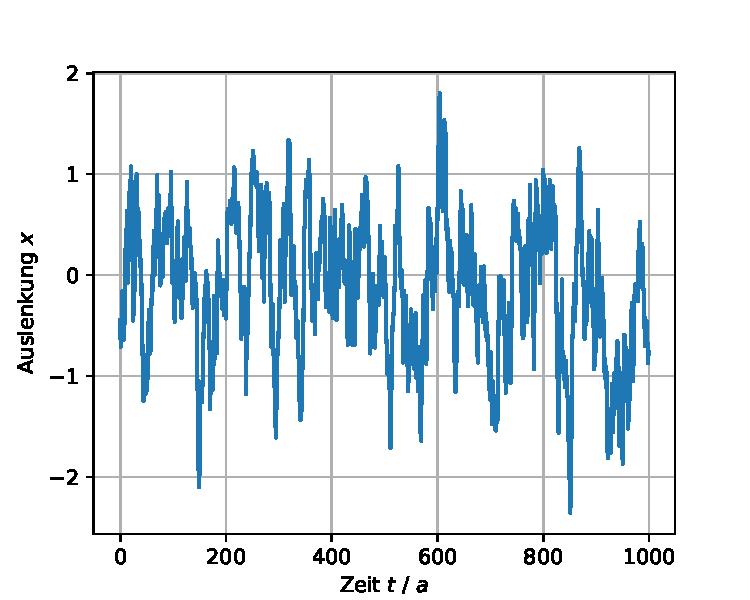
\includegraphics[width=.7\textwidth]{lasttrajectory}
    \caption{Ein Beispiel für eine Trajektorie des harmonischen Oszillators
    nach 10000 Sweeps des Metropolisalgorithmus'.}
    \label{fig:lastTrajectory}
\end{figure}

Um das zuvor Beschriebene etwas besser greifbar zu machen, soll es im Folgenden
kurz anhand des quantenmechanischen harmonischen Oszillators erläutert werden. Die
Wirkung des harmonischen Oszillators lautet nach Anwendung der
Wick-Rotation\footnote{Man bemerke den relativen Faktor $+1$ zwischen kinetischem
und Potentialterm, anders als im Fall mit Minkowski-Raumzeit!}
\[
    S[x] = \int_0^T \dd{t} \left\{ \frac{m}{2} \dot{x}(t)^2
    + \frac{\omega^2}{2} x(t)^2) \right\},
\]
Die Trajektorien $x$ werden einfach als eindimensionales Array gespeichert, der
Einfachheit halber nehmen wir $m=\omega=1$ an. Dann lautet die auf dem Gitter
formulierte, diskretisierte Version der Wirkung
\[
    S[x] = \frac{a}{2} \sum_{i=1}^{N} \left\{\left( \frac{x_i - x_{i-1}}{a} \right)^2
    + x_i^2 \right\}.
\]
Es ist klar, dass für $\Delta S[x'_i, x_i, x]$ nur wenige Terme aus dieser Summe
benötigt werden. In der Simulation wurden insgesamt 10000 Sweeps durchgeführt, wobei
das System \enquote{kalt}, also mit $x_i = 0 \, \forall x_i \in x$ initialisiert wurde.
Eine Trajektorie am Ende dieser 10000 Sweeps ist exemplarisch in Abb.
\ref{fig:lastTrajectory}
dargestellt. Es wird erwartet, dass sich das System nach vielen Iterationen im
Grundzustand befinden wird. Dies lässt sich durch folgende Überlegung motivieren:
Fügt man in den Propagator \eqref{eq:propagator} einen Einheitsoperator, ausgedrückt
durch die Energieeigenzustände, $\mathds{1} = \sum_n \ket{n} \bra{n}$, ein, so
ergibt sich
\begin{equation} \label{eq:groundStateAtLargeT}
    \bra{x_f} e^{-H t} \ket{x_i}
    = \sum_n \bra{x_f} e^{-H t} \ket{n} \braket{n}{x_i}
    = \sum_n e^{-E_n t} \braket{x_f}{n} \braket{n}{x_i}
    \xrightarrow{t \gg 1} e^{-E_0 t} \braket{x_f}{0} \braket{0}{x_i}.
\end{equation}
Für große $t$, d.\,h. hier nach vielen Iterationen, sollte das System im niedrigst
liegenden Energieeigenzustand liegen. Das wollen wir überprüfen, indem wir die
Energie sowie die Wellenfunktion des Zustands aus den Daten der Simulation
extrahieren.

\begin{figure}[htbp]
    \centering
    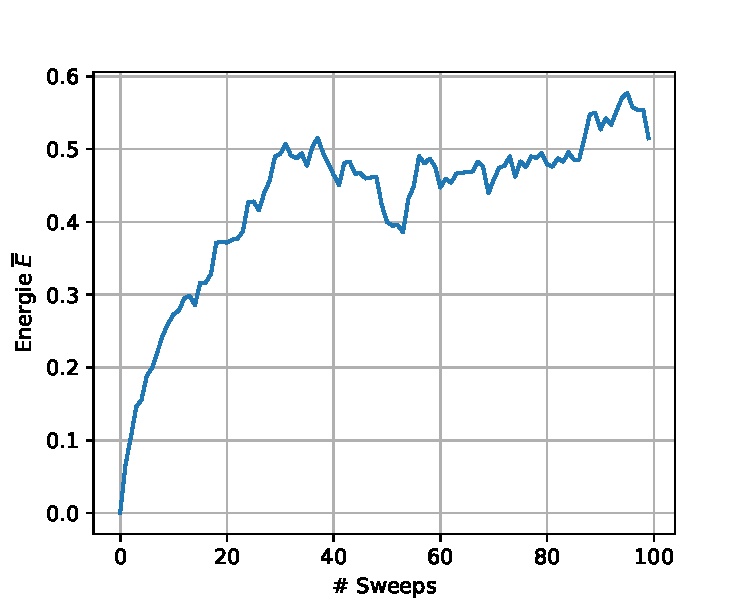
\includegraphics[width=.7\textwidth]{energies}
    \caption{Die gemessenen Energien $\overline{E}$ als Funktion der
    Monte-Carlo-Zeit. Es ist klar eine Konvergenz zu einem Plateau bei $\approx 0.5$
    erkennbar.}
    \label{fig:energies}
\end{figure}

Die Energie ist hier die simplere Sache: Hierfür messen wir zwischen den Sweeps
die Energie
\[
    \overline{E} = \hbar \omega \overline{x^2} = \overline{x^2},
\]
welche der Gesamtwirkung des Systems entspricht\footnote{$x$ ist die Position des
eindimensionalen harmonischen Oszillators. In dieser Rechnung wurde
der Virialsatz miteinbezogen: $T = \frac{1}{2} x V'(x)$. \cite{freedmanCreutz}}.
Das Ergebnis ist
in Abb. \ref{fig:energies} dargestellt: Zunächst ist deutlich sichtbar, wie das System
vom \enquote{kalten} Anfangszustand in den Gleichgewichtszustand konvergiert. Die
Werte zum Berechnen der Grundzustandsenergie nehmen wir ab 1000 Sweeps und
messen nur alle 50 Sweeps, um die Korrelation zwischen den Werten zu verringern.
Wir finden
\[
    \overline{\overline{E}} = 0.491 \pm 0.017,
\]
was den theoretischen Wert $E_0 = \hbar \omega (0 + \frac{1}{2}) = 0.5$
\cite{freedmanCreutz} in den Fehlerbereich miteinschließt. Hierbei wurde die
Unsicherheit auf die Messung durch den Standardfehler abgeschätzt.


\begin{figure}[htbp]
    \centering
    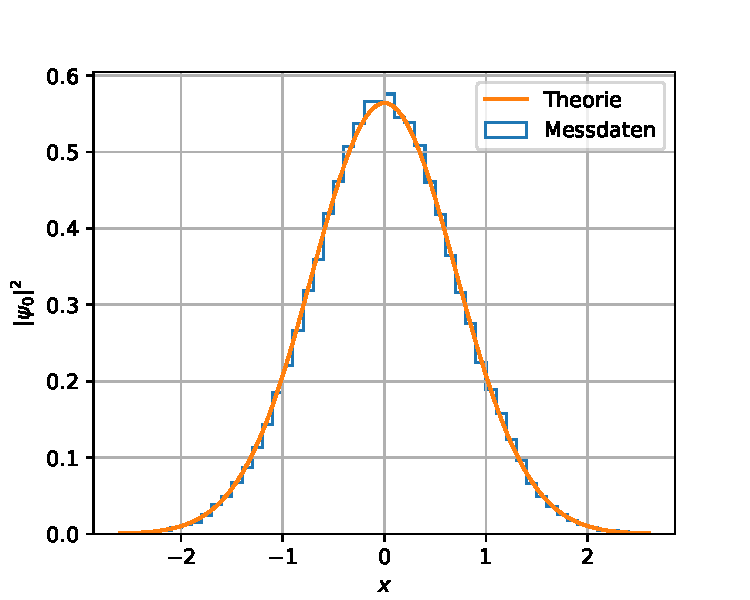
\includegraphics[width=.7\textwidth]{harmonicOscillatorDensity.pdf}
    \caption{Zustandsdichte des Grundzustands des harmonischen Oszillators.}
    \label{fig:harmonicOscDensity}
\end{figure}

Die Grundzustandswellenfunktion $\psi_0$ lässt sich zwar nicht als eine direkte
Observable messen, mittels eines Tricks können wir ihr Betragsquadrat $| \psi_0 |^2$
aber dennoch aus den Daten extrahieren. Hierfür nehmen wir einfach alle Positionen
aus allen Sweeps und stellen sie in einem Histogramm dar. Da $| \psi_0 |^2$ die
Wahrscheinlichkeitsdichte beschreibt, sollte das Histogramm ebendiese Verteilung
widerspiegeln. In Abb. \ref{fig:harmonicOscDensity} ist beides dargestellt, das
erwartete Verhalten ist eingetreten.

\section{Das SU(2)-Eichfeld auf einem Gitter}
\subsection{Yang-Mills}
Hauptbetrachtungsobjekt dieser Arbeit soll das Eichfeld $A_\mu$ der
SU(2)-Eichsymmetrie sein. Der Lagrangian der betrachteten Theorie enthält 
Terme
\[
    \overline{\psi}(x)(i \gamma^\mu \partial_\mu - m) \psi(x),
\]
bei $\psi$ handelt es sich also um ein fermionisches Feld\footnote{Hinzuzufügen
ist, dass es sich hierbei um eine stark vereinfachte Version handelt: In der
Realität wäre noch die Farbladung zu berücksichtigen~\cite{gattringerLang}.}.
Die betrachtete Eichtransformation wirkt auf die Felder dann wie folgt
\cite{gattringerLang}:
\[
    \psi(x) \mapsto \Omega(x) \psi(x), \; \Omega(x) \in \mathrm{SU}(2).
\]
Damit die Theorie eichinvariant wird, soll die Ableitung der Felder genauso
transformieren wie die Felder selbst und dafür muss $\partial_\mu$
durch eine kovariante Ableitung
\[
D_\mu = \partial_\mu + i A_\mu
\]
ersetzt werden. Hier ist $g$ die Kopplungsstärke. Das Eichfeld lässt sich in
seine Farbkomponenten zerlegen \cite{gattringerLang}
\[
    A_\mu = \frac{1}{2} \sum_{a = 1}^3 \tau^a A_\mu^a,
\]
wobei $\tau^a$ die Generatoren der Gruppe SU(2) sind. Im Rahmen dieser Arbeit
seien die Farbindizes stets unterdrückt, für eine explizitere Betrachtung sei
z.\,B. auf das Buch von Gattringer und Lang \cite{gattringerLang} verwiesen.
Als weitere Konvention wurde die Kopplungsstärke $g$ als Faktor in das Feld
absorbiert, daher taucht sie in der kovarianten Ableitung nicht
auf~\cite{gattringerLang}. 

Setzen wir nun als Transformationsverhalten für das Eichfeld
\[
    A_\mu(x) \mapsto \Omega(x) A_\mu(x) \Omega(x)^\dag
    + i \left( \partial_\mu \Omega(x) \right) \Omega(x)^\dag
\]
an \cite{gattringerLang}, so finden wir unter Verwendung von
$\Omega^\dag \Omega = \mathds{1}$
\begin{align*}
    D_\mu(x) \psi(x) \mapsto
    &\left( \partial_\mu + i \Omega(x) A_\mu \Omega(x)^\dag
    - \left( \partial_\mu \Omega(x) \right) \Omega(x)^\dag \right)
    \Omega(x) \psi(x)\\
    = &\left( \partial_\mu \Omega(x) \right) \psi(x)
    + \Omega(x) \partial_\mu \psi(x) + i \Omega(x) A_\mu(x) \psi(x)
    - \left( \partial_\mu \Omega(x) \right) \psi(x) \\
    = &\Omega(x) D_\mu(x) \psi(x).
\end{align*}
So kann also die Eichinvarianz der Theorie erreicht werden.

Die Dynamik des Eichfelds wird typischerweise durch die Yang-Mills-Wirkung
\begin{equation} \label{eq:yang-millsAction}
S[A] = \frac{1}{2 g^2} \int \dd^4{x} \, \mathrm{tr}\,
\left[ F_{\mu \nu}(x) F^{\mu \nu}(x) \right]
\end{equation}
beschrieben. \cite{gattringerLang} Hierbei ist
\[
F_{\mu \nu}(x) = -i [D_\mu(x), D_\nu(x)]
= \partial_\mu A_\nu(x) - \partial_\nu A_\mu(x) + i [A_\mu(x), A_\nu(x)]
\]
der Feldstärketensor. Hier ist die Kopplungskonstante $g$ dann explizit mit
notiert. Zunächst soll nun eine Version dieser Wirkung auf einem Gitter definiert
werden.

\subsection{Wilson}
Um die Integration über alle Dimensionen der Raumzeit zu implementieren,
brauchen wir ein vierdimensionales Gitter. Dieses Gitter habe in Zeitrichtung
eine Ausdehnung von $L_\mathrm{t}$ Gitterpunkten und in die drei Raumrichtungen
jeweils eine Ausdehnung von $L_\mathrm{s}$ Gitterpunkten. Wir verwenden
periodische Randbedingungen: Man kann das Gitter nicht \enquote{verlassen},
sondern läuft immer auf der gegenüberliegenden Seite wieder hinein. Befindet
man sich z.\,B. bei $(L_\mathrm{t}-1,0,0,0)$ und geht einen Schritt in
Zeitrichtung, so befindet man sich danach wieder bei $(0,0,0,0)$. Das Gitter
ist gewissermaßen in jeder Dimension an den Enden zusammengeklebt:
\[
\Lambda = \{0, 1, \dots, L_\mathrm{t}-1\}/(0 \sim L_\mathrm{t}-1)
\times \left( \{0, 1, \dots, L_\mathrm{s}-1 \} / (0 \sim L_\mathrm{s}-1) \right)^3,
\]
es handelt sich also um einen vierdimensionalen, diskretisierten Hypertorus.
Der Abstand der Gitterpunkte sei $a$; als Basis für das Gitter wählen wir die
Vektoren $a_\mu$, die von einem Gitterpunkt auf den nächsten in Richtung $\mu$
zeigen. Sie haben folglich die Länge $a$ und die Basis ist demnach keine
Ortho\emph{normal}basis.

Nun wollen wir unsere Felder auf dem Gitter definieren. Die kanonische
Entscheidung wäre, ihren Definitionsbereich auf das Gitter zu beschränken.
Leider zeigt sich bereits beim fermionischen Feld, dass das so einfach nicht
ist. Die diskretisierte Ableitung ließe sich z.\,B. so umsetzen:
\[
\partial_\mu \psi(x) = \frac{\psi(x + a_\mu) - \psi(x)}{a}.
\]
Betrachten wir dann das Verhalten so einer Ableitung unter der Eichtransformation,
so finden wir
\[
\partial_\mu(x) \psi(x) \mapsto
\frac{\Omega(x + a_\mu) \psi(x + a_\mu) - \Omega(x) \psi(x)}{a}.
\]
Dieses Ergebnis ist insofern problematisch, als dass wir durch die oben
so geschickt eingeführte kovariante Ableitung $D_\mu$ nicht das gewünschte
Transformationsverhalten erreichen können. Das liegt daran, dass hier
$\Omega$ an zwei verschiedenen Orten, $x$ und $x + a_\mu$, verwendet wird. Die
Lösung für dieses durch die Diskretisierung entstandene Problem findet sich in sog.
Paralleltransporten $U_\mu(x) \in \mathrm{SU}(2)$, deren Transformationsverhalten durch
\[
    U_\mu(x) \mapsto \Omega(x) U_\mu(x) \Omega(x + a_\mu)^\dag
\]
definiert ist~\cite{gattringerLang}. Verwenden wir dann die folgende neue kovariante
Ableitung
\[
    \tilde{D}_\mu \psi(x) =
    \frac{U_\mu(x) \psi(x + a_\mu) - \psi(x)}{a},
\]
so erhalten wir wieder das gewünschte Transformationsverhalten
\begin{align*}
    \tilde{D}_\mu \psi(x) \mapsto
    &\frac{\Omega (x) U_\mu(x)
    \overbrace{\Omega(x + a_\mu)^\dag \Omega(x + a_\mu)}^{= \mathds{1}}
    \psi(x + a_\mu) - \Omega(x) \psi(x)}{a} \\
    = & \Omega(x) \tilde{D}_\mu \psi(x).
\end{align*}
Die Paralleltransporte verdienen noch etwas Aufmerksamkeit: $U_\mu(x)$ kann als
\enquote{Zeiger} von $x$ nach $x + a_\mu$ interpretiert werden. Umgekehrt zeigt
$U_\mu(x)^\dag$ von $x + a_\mu$ auf $x$. \cite{urbachCPscript} Um die Verbindung
zum Eichfeld $A_\mu(x)$ herzustellen, reicht ein Blick auf ihre genaue
mathematische Definition \cite{gattringerLang}
\[
    U_\mu(x) = P \exp(i \int_\gamma \dd{s} A_\mu),
\]
hier ist $\gamma$ ein Pfad, der $x$ mit $x + a_\mu$ verbindet. Wenn man die
direkte Verbindungslinie für $\gamma$ annimmt und das Integral nun zu erster
Ordnung in $a$ auf dem Gitter ausführt, so findet man \cite{gattringerLang}
\begin{equation} \label{eq:parallelTransportexpA}
    U_\mu(x) = \exp(i a A_\mu(x)).
\end{equation}
Dieser Zusammenhang wird im Folgenden nützlich sein bei der Betrachtung der
Wilson-Wirkung, welche das Verhalten des Eichfelds auf einem Gitter beschreibt
\cite{urbachCPscript}:
\begin{equation} \label{eq:wilsonAction}
    S_\text{Wilson} = \frac{\beta}{2} \sum_{x \in \Lambda} \sum_{\mu < \nu}
    \text{Re} \; \text{tr} \left[\mathds{1} - U_{\mu \nu}(x) \right].
\end{equation}
Üblicherweise wird in dieser Formulierung die inverse Kopplung
$\beta = \frac{2 N_\text{c}}{g^2} = \frac{4}{g^2}$ verwendet. Was ist hier 
$U_{\mu \nu}$? Es handelt es sich um den kleinstmöglichen geschlossenen Ring von
Paralleltransporten \cite{urbachCPscript}
\[
    U_{\mu \nu}(x) = U_\mu(x) U_\nu(x + a_\mu) U_\mu(x + a_\nu)^\dag U_\nu(x)^\dag,
\]
der auch \emph{Plaquette} genannt wird. Man sieht leicht, dass die Spur\footnote{In
dieser Arbeit sind alle betrachteten Observablen $X$ die Spur einer Funktion 
von Paralleltransporten $X = \text{tr} \, Y$. Deswegen ist stets die Spur
$\text{tr} \, Y$ gemeint, auch wenn nur von $Y$ als Observable gesprochen wird.
Die Spur ist immer notwendig, um mit ihrer zyklischen Eigenschaft die Eichinvarianz
der Observablen zu erreichen.}
dieser Plaquette (wie die aller geschlossenen Ringe von Paralleltransporten)
eichinvariant ist, was auch die formulierte Wilson-Wirkung eichinvariant macht.
Nun wollen wir zeigen, dass die Wilson-Wirkung für kleine Gitterabstände $a$ wieder
in die Yang-Mills-Wirkung \eqref{eq:yang-millsAction} übergeht.

Dazu betrachten wir zunächst die Plaquette im Rahmen des oben gefundenen
exponentiellen Ausdrucks für die Paralleltransporte \eqref{eq:parallelTransportexpA}:
\begin{align*}
    U_{\mu \nu}(x) =
    &\exp(i a A_\mu(x)) \exp(i a A_\nu(x + a_\mu))
    \exp(-i a A_\mu(x + a_\nu)) \exp(-i a A_\nu(x)) \\
    = &\exp \left\{ i a \left(A_\mu(x)
    + A_\nu(x + a_\mu) - A_\mu(x + a_\nu)
    - A_\nu(x) \right) \right. \\
    &+ \frac{i a^2}{2} \left(-[A_\mu(x), A_\nu(x + a_\mu)]
    + [A_\mu(x), A_\mu(x + a_\nu)] \right. \\
    &+ [A_\mu(x), A_\nu(x)] + [A_\nu(x + a_\mu), A_\mu(x + a_\nu)] \\
    &+ \left. \left. [A_\nu(x + a_\mu), A_\nu(x)] \right) + \mathcal{O}(a^3) \right\} \\
    = &\exp{i a \cdot 0 + i a^2 \left(\partial_\mu A_\nu(x)
    -\partial_\nu A_\mu(x) + i [A_\mu(x), A_\nu(x)] \right) + \mathcal{O}(a^3)} \\
    = &\exp(i a^2 F_{\mu \nu}(x) + \mathcal{O}(a^3)).
\end{align*}
Hierbei wurde eine Version der Baker-Campbell-Hausdorff-Regel \cite{gattringerLang}
\[
    e^A e^B = e^{A + B + \frac{1}{2} [A, B] + \cdots}
\]
verwendet. Im zweiten Schritt wurden die Felder um $x$ entwickelt, also z.\,B.
\[
    A_\mu(x + a_\nu) = A_\mu(x) + a \partial_\nu A_\mu(x) + \mathcal{O}(a^2).
\]
Setzen wir das gefundene Ergebnis in die Wilson-Wirkung
\eqref{eq:wilsonAction} ein, so erhalten wir unter Berücksichtigung der
Antisymmetrie des Feldstärketensors \cite{gattringerLang}
\begin{align*}
    S_\text{Wilson} &= \frac{\beta}{2} \sum_{x \in \Lambda} \sum_{\mu < \nu}
    \text{tr} \left[\mathds{1} - \mathds{1}
    + \frac{1}{2} (a^2 F_{\mu \nu}(x))^2
    + \mathcal{O}(a^8) \right] \\
    &= \frac{a^4}{2 g^2} \sum_{x \in \Lambda} \text{tr} \left[ \sum_{\mu, \nu}
    (F_{\mu \nu}(x))^2 \right] + \mathcal{O}(a^8).
\end{align*}
Die Wilson-Wirkung bietet also eine ordentliche Annäherung an die im Kontinuum
formulierte Yang-Mills-Wirkung und kann für unsere Zwecke verwendet werden.

\subsection{Haar}
Für die Berechnung von Erwartungswerten auf dem Gitter wird ein Integrationsmaß
für die Paralleltransporte benötigt. Die naheliegende Wahl wäre \cite{gattringerLang}
\[
    \mathscr{D}[\mathcal{U}] = \prod_{x \in \Lambda} \prod_{\mu = 0}^3 \dd{U_\mu(x)}.
\]
Hier ist $\mathcal{U} = \{U_\mu(x) \, | x \in \Lambda, \mu \in \{0,1,2,3\}\}$ die
Menge aller Paralleltransporte auf dem Gitter. Hiermit finden wir also z.\,B.
\[
    Z = \int \mathscr{D}[\mathcal{U}] e^{-S_\text{Wilson}[\mathcal{U}]}.
\]
Auch für diese Größe wollen wir die Eigenschaft der Eichinvarianz ansetzen können,
damit die schlussendlich berechneten Erwartungswerte ebenfalls eichinvariant sind.
Da die Wilson-Wirkung bereits eichinvariant ist, muss also folgendes gelten:
\[
    \dd{U'_\mu(x)} = \dd{\left( \Omega(x) U_\mu(x) \Omega(x + a_\mu)^\dag \right)}
    \overset{!}{=} \dd{U_\mu(x)}.
\]
Der perfekte Kandidat für dieses Problem ist das sog. Haar-Maß, welches für Elemente
einer Gruppe $U, V \in G$ definiert ist und folgende Bedingungen erfüllen muss
\cite{gattringerLang}:
\[
    \dd{(U V)} = \dd{(V U)} = \dd{U}, \; \int \dd{U} = 1.
\]
Für eine etwas detailliertere Diskussion dieses Themas sei auf das Buch von
Gattringer und Lang \cite{gattringerLang} verwiesen, hier soll uns genügen, dass
das Integrationsmaß die genannten Bedingungen erfüllt und so unsere Erwartungswerte
eichinvariant macht.

\subsection{Wilson und Metropolis} \label{sec:wilsonMetropolis}
Um den Metropolisalgorithmus auf dem Gitter umsetzen zu können, fehlt uns noch eine
effiziente Methode, um $\Delta S$ zu berechnen. Es ist einleuchtend, dass die durch
die Veränderung eines einzelnen Paralleltransports $U_\mu(x)$ modifizierten Plaquettes
ebenjene sind, an denen $U_\mu(x)$ als \enquote{Kante} beteiligt ist. Je Ebene
$(\mu, \nu)$ in der Raumzeit gibt es hiervon zwei -- \enquote{oberhalb} und
\enquote{unterhalb} von $U_\mu(x)$. Wir finden also
\begin{align*}
    \Delta S &= -\frac{\beta}{2} \sum_{\nu \neq \mu} \mathrm{tr} \left[ \right.
        U'_{\mu \nu}(x) - U_{\mu \nu}(x)
        + U'_{\mu \nu}(x - a_\nu) - U_{\mu \nu}(x - a_\nu) \left. \right] \\
    &= -\frac{\beta}{2} \sum_{\nu \neq \mu} \mathrm{tr} \left[ \right.
        U'_{\mu \nu}(x) - U_{\mu \nu}(x)
        + (U'_{\mu \nu}(x - a_\nu) - U_{\mu \nu}(x - a_\nu))^\dag \left. \right] \\
    &= -\frac{\beta}{2} \sum_{\nu \neq \mu} \mathrm{tr} \left[ \right.
       (U'_\mu(x) - U_\mu(x)) U_\nu(x + a_\mu) U_\mu(x + a_\nu)^\dag U_\nu(x)^\dag \\
    & \qquad \qquad + U_\nu(x - a_\nu) (U'_\mu(x) - U_\mu(x))
    U_\nu(x + a_\mu - a_\nu)^\dag U_\mu(x - a_\nu)^\dag \left. \right] \\
    &= -\frac{\beta}{2} (U'_\mu(x) - U_\mu(x)) \sum_{\nu \neq \mu}
    \text{tr} \left[ \right. U_\nu(x + a_\mu) U_\mu(x + a_\nu)^\dag U_\nu(x)^\dag \\
    & \qquad \qquad \qquad  \qquad \underbrace{\qquad+ U_\nu(x + a_\mu - a_\nu)^\dag
    U_\mu(x - a_\nu)^\dag
    U_\nu(x - a_\nu) \left. \right]}_{\eqqcolon K_{\mu \nu}(x)}.
\end{align*}
Hier wurde im zweiten Schritt
$\text{tr} \, U = \text{tr} \, U^\dag \; \forall U \in \text{SU}(2)$
und im dritten Schritt die Zyklizität der Spur verwendet. Die Größe $K_{\mu \nu}(x)$
wird \emph{staple} genannt. Wie zuvor angedeutet, muss also für die Berechnung von
$\Delta S [U'_\mu(x), U_\mu(x), \mathcal{U}]$ nicht das gesamte Gitter berücksichtigt
werden, es
genügt die Betrachtung der $3 \cdot 6 = 18$ umliegenden Paralleltransporte.


\subsection{Das statische Potential und Wilson-Loops} \label{sec:thWilsonLoops}
Eine wichtige Observable auf dem Gitter sind sog. Wilson-Loops, die geschlossene
Ringe von Paralleltransporten darstellen. Im einfachsten Fall kann man sie sich
als Rechteck vorstellen:
\[
    W(x, \mu, \nu, m, n) = \text{tr} \left[ L(x, \mu, m)
    \cdot L(x + m a_\mu, \nu, n) \cdot L(x + n a_\nu, \mu, m)^\dag
    \cdot L(x, \nu, n)^\dag \right],
\]
\[
    L(x, \mu, m) = \prod_{i=0}^{m-1} U_\mu(x + i a_\mu)
\]
Man erkennt gut, dass es sich hierbei um die Verallgemeinerung der zuvor besprochenen
Plaquette $U_{\mu \nu}(x)$ handelt.
Im folgenden soll motiviert werden, dass sich aus dem Erwartungswert
$\langle W(0, i, l_\text{t}, l_\text{s}) \rangle =: \langle W(r,t)\rangle$
das Potential zweier unendlich schwerer, immobiler (\enquote{statischer}) Quarks mit
Abstand $r = l_\text{s} a$ extrahieren lässt.

Ausgangspunkt ist die Überlegung \eqref{eq:groundStateAtLargeT}, welche wir beim
harmonischen Oszillator angestellt haben: Für große Zeiten $t$ wird ein
physikalisches System im Rahmen des Feynman'schen Pfadintegralformalismus stets
auf den mit dem Grundzustand überlappenden Zustand übergehen. Nun ist also das Ziel,
einen Quark-Antiquark-Paar-Zustand zu erzeugen, der bei konstantem Ort durch die
Zeit propagiert und dann wieder annihiliert wird.

Die naheliegende Entscheidung liegt in einer Kombination des Propagators eines
unendlich schweren Quarks an einer konstanten Position $x$ \cite{latticeQCDforNovices}
\[
    G_\infty(t, \vec{x}) = U_0(t-a, \vec{x})^\dag U_0(t-2a, \vec{x})^\dag
    \dots U_0(0, \vec{x})^\dag
\]
mit dem eines unendlich schweren Antiquarks, $G_\infty(t, \vec{y})^\dag$. Hier haben
wir bereits zwei \enquote{Kanten} des späteren Wilson-Loops. Um das Konstrukt
eichinvariant zu machen, fügen wir zwei weitere Kanten hinzu, die $(0,\vec{x})$
und $(0,\vec{y})$ bzw. $(t,\vec{x})$ und $(t,\vec{y})$
verbinden.\footnote{Hier sei hinzugefügt, dass diese beiden Kanten sich jederzeit
durch sog. \emph{gauge fixing} wieder \enquote{entfernen} lassen, vgl. hierfür z.\,B. 
\cite{gattringerLang}.} So haben wir die zuvor definierten Wilson-Loops wiedergefunden
und finden für ihren Erwartungswert \cite{loopsStaticPotRothe}
\begin{equation} \label{eq:wilsonStaticPot}
    \langle W(r,t) \rangle = C \cdot e^{-t V(r)}.
\end{equation}
Im weiteren Verlauf dieser Arbeit werden wir also Wilson-Loops verschiedener Maße
$\overline{W(r,t)}$ messen und durch Anpassungen von exponentiellen Modellen an die
gewonnenen Daten das statische Potential extrahieren. Es ist auch möglich, sog.
\emph{nichtplanare} Wilson-Loops zu vermessen, also solche, die nicht der oben
benannten, rechteckigen Form entsprechen. So ist es möglich, auch nichtganzzahlige
Abstände $r$ zu vermessen.

Die hier vorgenommene Diskussion dieser Observablen erhebt keinerlei Anspruch auf
Vollständigkeit oder Rigorosität. Eine in dieser Hinsicht bessere Betrachtung ist
im Buch von Rothe \cite{loopsStaticPotRothe} zu finden. 
